\documentclass[12pt,aspectratio=169]{beamer}

\usetheme{metropolis}

\definecolor{mDarkBrown}{HTML}{FF5722}
\definecolor{mDarkTeal}{HTML}{263238}
\definecolor{mLightBrown}{HTML}{FF5722}

\usepackage{booktabs}
\usepackage{graphicx}
\usepackage{hyphenat}
\usepackage{multirow}
\usepackage{nicefrac}
\usepackage[normalem]{ulem}

\usepackage{pifont}
\newcommand{\cmark}{\ding{51}}
\newcommand{\xmark}{\ding{55}}

\usepackage{minted}
\usemintedstyle{tango}
\newminted[bash]{bash}{%
    autogobble,
    bgcolor=mDarkTeal!10,
    linenos
}
\newminted[py3]{python}{%
    python3,
    autogobble,
    bgcolor=mDarkTeal!10,
    linenos
}
\newminted[sql]{sql}{%
    autogobble,
    bgcolor=mDarkTeal!10,
    linenos
}

\usepackage{polyglossia}
\setdefaultlanguage[variant=british]{english}
\usepackage[english=british]{csquotes}

\defaultfontfeatures{Ligatures=TeX}
\setmainfont{Lucida Sans OT}
\setsansfont[Scale=MatchLowercase]{Lucida Sans OT}
\setmonofont[Scale=MatchLowercase]{Lucida Console DK}

\usepackage{mathspec}
\setmathsfont(Digits,Latin,Greek)[Numbers={Lining,Proportional}]{Lucida Bright Math OT}

\newcommand{\mat}[1]{\ensuremath{\mathbf{#1}}}

\newcommand{\R}{\ensuremath{\mathbb{R}}}

\newcommand{\E}[1]{\ensuremath{\mathbb{E}\!\left[ #1 \right]}}
\newcommand{\V}[1]{\ensuremath{\mathbb{V}\!\left[ #1 \right]}}
\newcommand{\Prob}[1]{\ensuremath{\Pr\!\left( #1 \right)}}
\newcommand{\Normal}[2]{\ensuremath{\mathcal{N}\!\left( #1, #2 \right)}}
\newcommand{\simiid}{\ensuremath{\overset{\text{\tiny i.i.d.}}{\sim}}}

\DeclareMathOperator{\logit}{logit}

\author{Gianluca Campanella}
\date{}



\title{Introduction to Data Science}

\begin{document}

\maketitle

\begin{frame}{Contents}
    \tableofcontents[hideallsubsections]
\end{frame}

\section{What is Data Science?}

\begin{frame}{What is Data Science?}
    \only<1>{%
        \begin{columns}
            \begin{column}{0.5\textwidth}
                \begin{center}
                    Mathematics and \\ Statistics / Operational Research
                \end{center}
            \end{column}
            \begin{column}{0.5\textwidth}
                \begin{center}
                    Computing and \\ Software Engineering
                \end{center}
            \end{column}
        \end{columns}
        \vfill
        \begin{columns}
            \begin{column}{0.5\textwidth}
                \begin{center}
                    Visualisation and \\ Communication Skills
                \end{center}
            \end{column}
            \begin{column}{0.5\textwidth}
                \begin{center}
                    Domain expertise
                \end{center}
            \end{column}
        \end{columns}}
    \only<2>{%
        \begin{center}
            \LARGE%
            A \alert{problem\hyp{}solving approach} \\
            based on the scientific method
        \end{center}}
\end{frame}

\begin{frame}[t]{What does Data Science deal with?}
    \only<1>{%
        \begin{center}
            \LARGE%
            Problems!
        \end{center}
        \vfill
        Can we \alert{improve}\ldots\vspace{-1ex}
        \begin{itemize}
            \item The quality of offers we send to our customers?
            \item Road safety?
            \item How we identify people at high risk of cancer?
        \end{itemize}}
    \only<2>{%
        \begin{center}
            \LARGE%
            Predictions?
        \end{center}
        \vfill
        \alert{How likely}\ldots\vspace{-1ex}
        \begin{itemize}
            \item Is a customer to respond to some offer?
            \item Are traffic accidents to occur in a certain area?
            \item Is a person to develop cancer in the next 10 years?
        \end{itemize}}
    \only<3>{%
        \begin{center}
            \LARGE%
            Mechanisms?
        \end{center}
        \vfill
        \alert{Why}\ldots\vspace{-1ex}
        \begin{itemize}
            \item Does a customer decide to respond to some offer?
            \item Do traffic accidents occur regularly in certain areas?
            \item Do people develop cancer?
        \end{itemize}}
\end{frame}

\begin{frame}{What is Data Science?}
    \only<1>{%
        \vspace{0.5em}
        \begin{block}{Statistics}\vspace{-0.25em}
            \begin{itemize}
                \item Predates computers
                \item \alert{Understand why something happens} in the face of
                      uncertainty
            \end{itemize}
        \end{block}
        \vfill
        \begin{block}{Machine Learning}\vspace{-0.25em}
            \begin{itemize}
                \item `Algorithmic modelling' (L. Breiman)
                \item Computers can \alert{learn rules} without explicit
                      programming
            \end{itemize}
        \end{block}
        \vfill
        \begin{block}{Deep Learning}\vspace{-0.25em}
            \begin{itemize}
                \item Less structured inputs
                \item Computers can \alert{learn structure} without explicit
                      programming
            \end{itemize}
        \end{block}}
    \only<2>{%
        \begin{columns}[c]
            \begin{column}{0.25\textwidth}
            \end{column}
            \begin{column}{0.375\textwidth}
                \begin{center}
                    \Large\bf%
                    Predictions
                \end{center}
            \end{column}
            \begin{column}{0.375\textwidth}
                \begin{center}
                    \Large\bf%
                    Mechanisms
                \end{center}
            \end{column}
        \end{columns}
        \vfill
        \begin{columns}[c]
            \begin{column}{0.25\textwidth}
                \begin{center}
                    \Large\bf%
                    Analysis
                \end{center}
            \end{column}
            \begin{column}{0.375\textwidth}
                \begin{center}
                    \textbf{Descriptive} \\
                    What's happening?
                \end{center}
            \end{column}
            \begin{column}{0.375\textwidth}
                \begin{center}
                    \textbf{Diagnostic} \\
                    Why is it happening?
                \end{center}
            \end{column}
        \end{columns}
        \vfill
        \begin{columns}[c]
            \begin{column}{0.25\textwidth}
                \begin{center}
                    \Large\bf%
                    Building
                \end{center}
            \end{column}
            \begin{column}{0.375\textwidth}
                \begin{center}
                    \textbf{Predictive} \\
                    What's likely to happen?
                \end{center}
            \end{column}
            \begin{column}{0.375\textwidth}
                \begin{center}
                   \textbf{Prescriptive} \\
                   What do I need to do?
                \end{center}
            \end{column}
        \end{columns}}
\end{frame}

\begin{frame}{Recap}
    \begin{block}{Data Science is\ldots}
        \begin{itemize}
            \setlength{\itemsep}{0.75em}
            \item \alert{Evidence\hyp{}based problem solving and
                         decision\hyp{}making}
            \item Multidisciplinary but domain\hyp{}driven
            \item Analysis\hyp{}focused or building\hyp{}focused
        \end{itemize}
    \end{block}
\end{frame}

\section{Who is a Data Scientist?}

\begin{frame}{Who is a Data Scientist?}
    Someone who can\ldots
    \begin{itemize}
        \setlength{\itemsep}{0.75em}
        \item Get a `feel' for the data
        \item Communicate effectively
        \item Work well in a team
    \end{itemize}
\end{frame}

\begin{frame}{What's this `feel' for the data?}
    \only<1>{%
        \begin{itemize}
            \setlength{\itemsep}{0.75em}
            \item Passion for the domain
            \item Curiosity about the data
            \item Intuition and creativity
            \item Common sense
            \item Rigour and accuracy
            \item Relevance
        \end{itemize}}
    \only<2>{%
        \begin{center}
            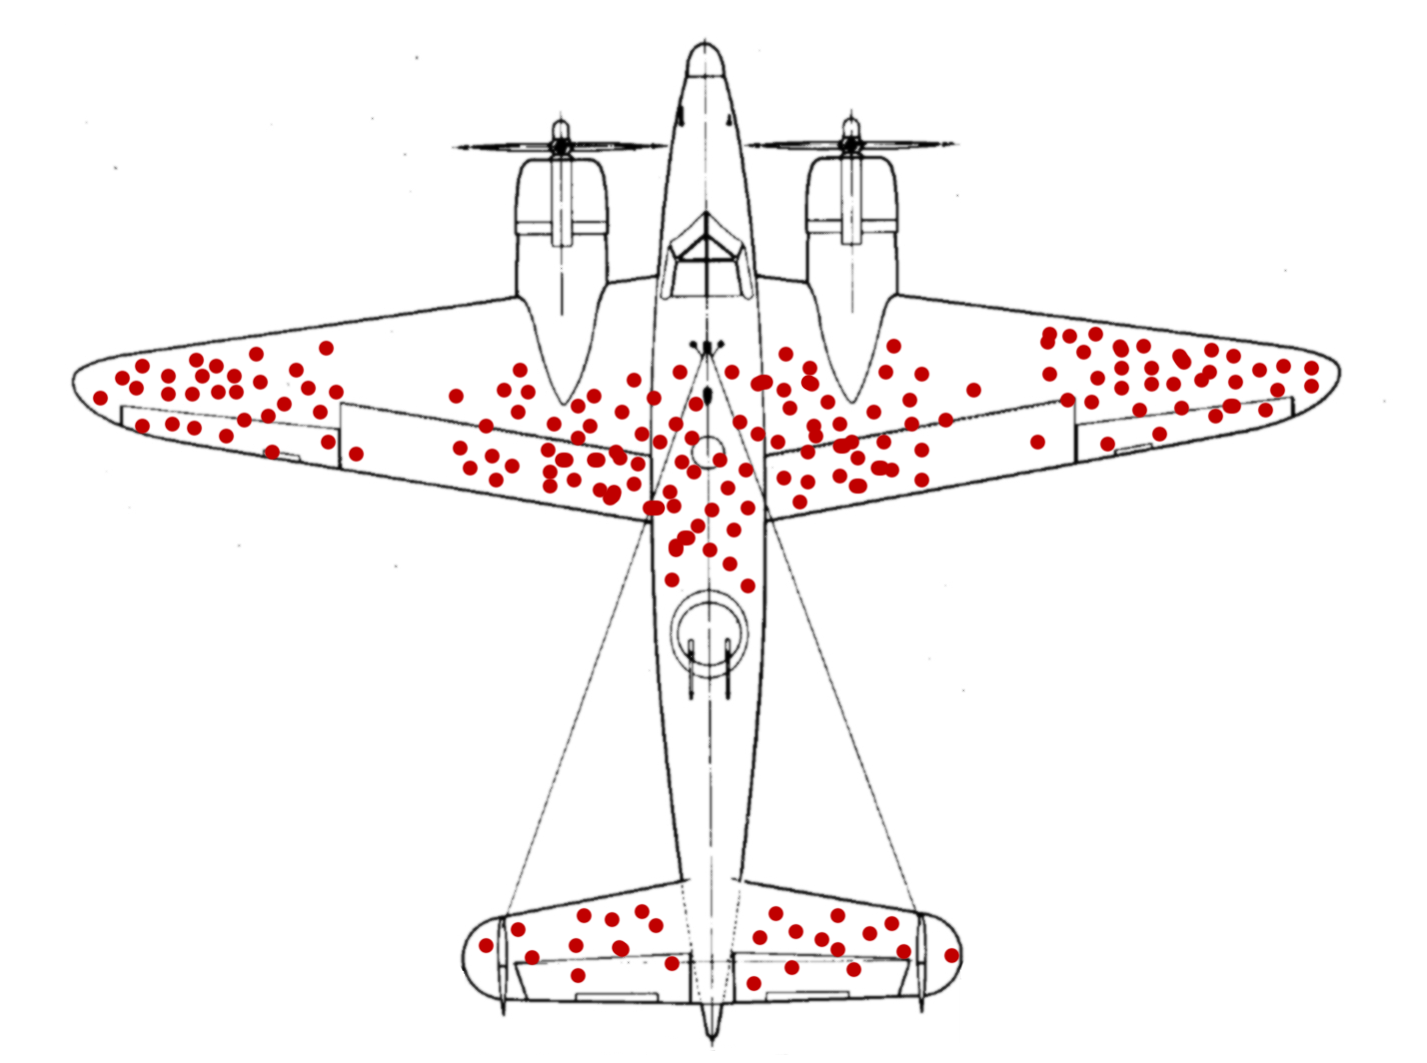
\includegraphics[height=0.8\textheight]{figures/survivorship_bias} \\
            {\scriptsize%
             Via \textit{Wikimedia Commons}}
        \end{center}}
\end{frame}

\begin{frame}{How do I communicate effectively?}
    \only<1>{%
        \begin{itemize}
            \setlength{\itemsep}{0.75em}
            \item Condense findings into \alert{recommendations}
            \item Use \alert{storytelling} techniques and \alert{visual aids}
            \item Understand limitations and \alert{don't overstate results}
        \end{itemize}}
    \only<2>{%
        \begin{center}
            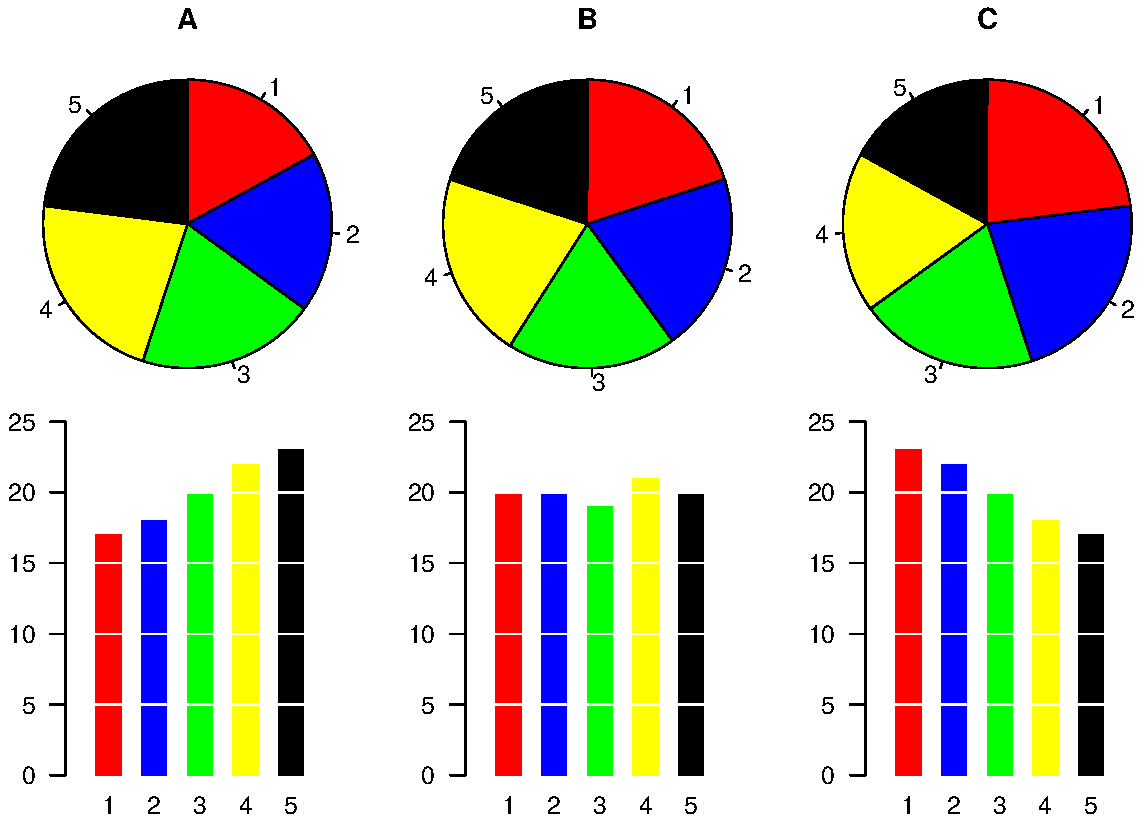
\includegraphics[height=0.8\textheight]{figures/pies} \\
            {\scriptsize%
             Via \textit{Wikimedia Commons}}
        \end{center}}
\end{frame}

\begin{frame}{Recap}
    A successful Data Scientist\ldots
    \begin{itemize}
        \item Is insatiably curious --- and a bit stubborn!
        \item Never stops learning
        \item Is a practical, impact\hyp{}driven, dependable person
        \item Can tell a story
        \item Knows the limitations of Data Science
    \end{itemize}
\end{frame}

\end{document}

